% The following file houses the System Requirements for Apex Automation's Pill Dispenser. All intellectual property belongs to the authors denoted on the document.

%Usually an article, 12pt font, with a separate title page
\documentclass[12pt]{article}
\usepackage{preamble}
\usepackage{caption}
\captionsetup{skip=0pt}

\begin{document}

% Edit title page in the titlepage.tex file.
% This title page template belongs to Apex Automation and may not be used without their consent.



% Please fill out the following information.
\newcommand{\org}{McMaster University}   % Enter name of organization
\newcommand{\headingmajor}{MECHTRON 4TB6A}   % Enter the major heading
\newcommand{\headingminor}{Mechatronics \& Software Engineering Capstone}   % Enter the minor heading
\newcommand{\doctitle}{System Requirements}   % Enter the title of the document
\newcommand{\projtitle}{Health Mate - Pill Dispenser}   % Enter the project title
\newcommand{\logofile}{ApexEngineering.png}   % Enter the file name for team logo
\newcommand{\projdate}{Sunday, November 1, 2020}   % Enter the date



%--------------Do not touch below this line unless you intent to change format, spacing, etc.-----------------
\begin{titlepage}

% Defines a new command for the horizontal lines, change thickness here
\newcommand{\HRule}{\rule{\linewidth}{0.5mm}}

% Center everything on the page
\center

% HEADING SECTIONS
\textsc{\LARGE \org}\\[1.5cm] % Name of your university/organization
\textsc{\Large \headingmajor}\\[0.5cm] % Major heading such as course name
\textsc{\large \headingminor}\\[0.5cm] % Minor heading such as course title

% TITLE SECTION
\vspace{1cm}
\HRule \\[0.2cm]
{ \Large \vspace{0.25cm}  \textsc{  \LARGE \doctitle} \vspace{0.3cm} }  % Title of your document
\HRule \vspace{.5cm}
\textsc{\LARGE \projtitle} % Project title
\vspace{1cm}
% Firm/Team logo included here. 
 \begin{figure}[h]
  \centering
  \includegraphics[width=.4\linewidth]{\logofile}
\end{figure}
 \vspace{1cm}
 
% AUTHOR SECTION
\begin{table}[ht!] \centering
\begin{tabular}{c c c}
\toprule
\textbf{Name} & \textbf{Student Number} & \textbf{McMaster Email} \\ 
\midrule
Justin Ballaro & 400015482 & ballaroj@mcmaster.ca \\
Joel Bates & 001420696 & batesjj@mcmaster.ca \\
Brodie Bresette & 400029059 & bresettb@mcmaster.ca \\
Nicholas D'Angelo & 400018631 &  dangelon@mcmaster.ca  \\
Daniel Pietrangelo & 400010287 &  pietrand@mcmaster.ca \\
\bottomrule
\end{tabular}
\label{Tab:HU}
\end{table}

% DATE SECTION
%{\large \projdate}\\[3cm] % Date exlcude b/c it is available in the revisions table.
\end{titlepage}
 
\pagebreak
% header and footer settings
\pagestyle{fancy} \fancyhf{}
\lhead{\fontsize{10pt}{10pt}\selectfont System Requirements} \rhead{\fontsize{10pt}{10pt}\selectfont Revision \rev} \cfoot{\thepage}

% Edit table of revisions in tableofrevisions.tex
\pagenumbering{roman}


\newcommand{\rev}{0}  %-------INSERT MOST RECENT REVISION NUMBER HERE

\section*{Table of Revisions}
\begin{table}[ht!]
\begin{center}
\begin{adjustbox}{max width=\textwidth}
\small
\begin{tabular}{|p{0.1\textwidth}|p{0.15\textwidth}|p{0.2\textwidth}|p{0.4\textwidth}|}
 \hline
 \textbf{Revision } & \textbf{Date} &
 \textbf{Authors} &
 \textbf{Revision Comments}\\
 \hline \centering
 0 & \centering
 17/02/2021 & 
 Justin Ballaro \newline
Joel Bates \newline
Brodie Bresette \newline
Nicholas D'Angelo \newline
Daniel Pietrangelo &
Inital Revision \\
\hline
\end{tabular}
\end{adjustbox}
\end{center}
\caption{Table of Revisions}
\end{table}

\pagebreak
\tableofcontents
\listoffigures
\listoftables
\pagebreak
\pagenumbering{arabic}

%----------Begin adding text here.----------

\section{Introduction}
\subsection{Document Purpose}
The purpose of this document is to define the minimum functional requirements for the Healthmate pill dispenser system. Meeting these requirements is the driving force behind system design and is a key success criteria for the project. These requirements are referenced in the System Design and Validation \& Verification documents.


\subsection{Project Purpose \& Scope}
The medication taken by an individual is only as effective as the abidance by the patient to take the prescribed medication at the times designated. The purpose of this project is to develop an integrated hardware and software system to improve the medication adherence for users who receive their prescriptions in sachet/pouch style packaging. This device will focus on dispensing PACMED pouches developed by McKesson Corporation. \par
The system to be implemented will provide real time alarms/reminders when it is time for the user to take their medication. The system will also dispense the user's medication in such a manor as to make it easy to retrieve and ingest. Once a scheduled dose has been taken/missed the system will record adherence data. This data will be stored locally on the device.\par
This project's scope consists of four main components. A general overview of each component can be found below:
\begin{enumerate}
    \item System to insert strip packaged medication into the device.
    \item System for dispensing individual packages from a strip package.
    \item Embedded control system that initiates dispensing, reads user interactions, and collects data.
    \item User interface for user information and settings control.
\end{enumerate}


\subsection{Operational Overview}
A individual will insert their PACMED strip package into the device, aligning the first pouch with an alignment groove. After insertion they will be prompted to set their preferred dispensing times within predefined ranges for morning, lunch, supper and bedtime doses. When it is time for a scheduled dose an audible alarm will activate. Upon alarm acknowledgement, the device will cut open and dispense the required pouch/pouches, and the user can freely remove their medication from the device. Under normal operation, dispensing events will continue to occur at the specified times until all pouches have been dispensed from the device. \par
The user may interact with an interface on the device. Through this interface they will be able to modify the dispensing schedule, initiate manual dispense requests and view adherence data.

\pagebreak

\section{Definitions \& Naming Conventions}

\subsection{General Definitions}
\begin{table}[htb!]
\begin{center} \begin{adjustbox}{max width=\textwidth}\small
\begin{tabular}{|p{0.15\textwidth}|p{0.75\textwidth}|}
 \hline
 \textbf{Word} & \textbf{Definition}\\
 \hline 
 Healthmate & The name of the dispensing device. Any reference to ``Healthmate'' is referring to the entire pill dispensing system.   \\ \hline
 PACMED Strip Package & Medication storage/adherence product sold my McKesson Corporation. It is a box containing a filled strip pack (see strip pack below). \\ \hline
 Strip Pack & A series of filled medication pouches attached by the seam in a single continuous strip. \\ \hline
 Pouch & An sealed package containing a single dose of medication. These pouches have the date and either MORNING, LUNCH, SUPPER or BEDTIME written on them, indicating when the medication inside should be consumed. \\ \hline
 Sachet &  Another word to describe a pouch (see pouch above). \\ \hline
 Dispense &  The action of cutting open open a pouch and making it available for collection. \\ \hline
 Collection & The end user removing an opened pouch from the device. \\ \hline
 Adherence Data & Data indicating the date and time when a pouch has been dispense, as well as, the date and time when the pouch is collected. \\ \hline
\end{tabular}\end{adjustbox}\end{center}\caption{General definitions.}
\end{table}


\subsection{Naming Conventions}
\begin{table}[htb!] \begin{center} \begin{adjustbox}{max width=\textwidth} \small
\begin{tabular}{|p{0.15\textwidth}|p{0.3\textwidth}|}
 \hline
 \textbf{Prefix} & \textbf{Description}\\
 \hline 
 m\_ & Monitored variable.\\ \hline
 c\_ & Controlled variable.\\ \hline
 k\_ & Constant variable.\\ \hline
 FR\# & Functional requirement.\\ \hline
 NFR\# & Non-functional requirement.\\ \hline
\end{tabular} \end{adjustbox} \end{center}
\caption{Naming conventions.}
\end{table}

\pagebreak

\subsection{Constants} 
\begin{table}[htb!] \begin{center} \begin{adjustbox}{max width=\textwidth}
\small
\begin{tabular}{|p{0.3\textwidth}|p{0.4\textwidth}|p{0.10\textwidth}|p{0.10\textwidth}|}
 \hline
 \textbf{Name} & \textbf{Description} & \textbf{Value} & \textbf{Units}\\
 \hline 
 k\_DispenserLength & The length of Healthmate. & TBD & cm\\
 \hline
 k\_DispenserWidth & The width of Healthmate. & TBD & cm\\
 \hline
 k\_DispenserHeight & The height of Healthmate. & TBD & cm\\
 \hline
 k\_StripPackageLength & The length of the PACMED Strip Package. & 10.8 & cm\\
 \hline
 k\_StripPackageWidth & The width of the PACMED Strip Package. & 7.6 & cm\\
 \hline
 k\_StripPackageHeight & The height of the PACMED Strip Package. & 10.8 & cm\\
 \hline
 k\_PouchLength & The length of a single pouch. & 7.5 & cm\\
 \hline
 k\_PouchWidth & The width of a single pouch. & 7.0 & cm\\
 \hline
\end{tabular} \end{adjustbox} \end{center}
\caption{Constant variables.}
\end{table}


\subsection{Monitored Variables}
\begin{table}[htb!] \begin{center} \begin{adjustbox}{max width=\textwidth}
\small
\begin{tabular}{|p{0.3\textwidth}|p{0.5\textwidth}|p{0.10\textwidth}|}
 \hline
 \textbf{Name} & \textbf{Description} & \textbf{Units}\\
 \hline 
m\_PillCollected & Whether or not the medication has been taken from the dispenser. & bool\\
 \hline
m\_PillDispensed & Tracks when pills are physically dispensed. True if pills make it to the collection area  & bool\\
 \hline
m\_DispensingSchedule & Schedule of when pills will be dispensed (default or user inputted times). & json string \\
 \hline
m\_StripPackageSeated & Whether or not the strip package has been inserted and aligned correctly. & bool \\
 \hline
m\_DateTime & Needed to follow medication schedule. & dd:mm:yy hh:mm:ss\\
 \hline
m\_UserInputs & Result of users interaction with the UI, could be manual dispense requests, schedule change, clock change, view adherence stats & N/A\\
 \hline
\end{tabular} \end{adjustbox} \end{center} 
\caption{Monitored variables.} 
\end{table}

\pagebreak

\subsection{Controlled Variables}
\begin{table}[htb!] \begin{center} \begin{adjustbox}{max width=\textwidth} \small
\begin{tabular}{|p{0.3\textwidth}|p{0.5\textwidth}|p{0.10\textwidth}|}
 \hline
 \textbf{Name} & \textbf{Description} & \textbf{Units}\\
 \hline 
 c\_AdherenceStatistics & Data collected on taken/missed pills. & json string\\
 \hline
 c\_AudioVisualAlarm & Cue for user to take medication. & bool \\
 \hline
 c\_DispensingMechanism & Dispenses the appropriate pouch/pouches when scheduled. & N/A \\
 \hline
 c\_SeatedErrorNotifier & Lets user know if the strip package has not been inserted and aligned properly. & bool\\
 \hline
\end{tabular}\end{adjustbox} \end{center}
\caption{Controlled variables}
\end{table}


\section{System Overview}

\subsection{Context Diagram}
The following is a context diagram defining the boundaries between the system and the environment.
 \begin{figure}[htp!]
  \centering
  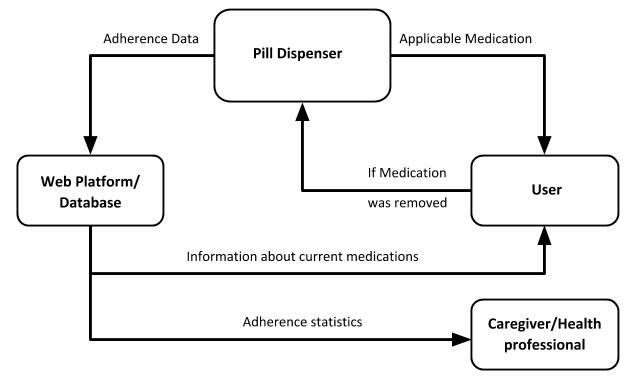
\includegraphics[width=1\linewidth]{ContextDiagram.jpg}
  \caption{Context Diagram}
\end{figure}


\subsection{Functional Decomposition}
\begin{figure}[!htbp]
    \centering
    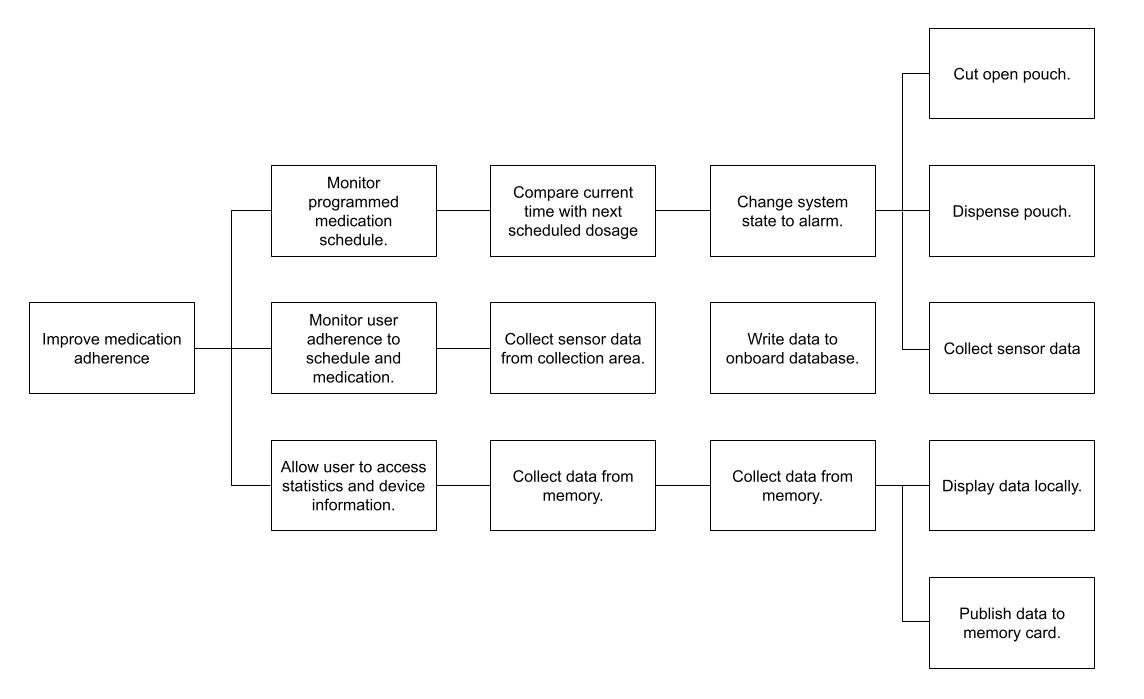
\includegraphics[width=\textwidth,height=\textheight,keepaspectratio]{project_requirements/FuncDecomp.jpg}
    \caption{Functional Decomposition Diagram}
    \label{fig:my_label}
\end{figure}
%NEED TO ADD A DESCRIPTION TO FOLLOW UP ON THE FUNCTIONAL DECOMPISTION --> see AVCS example

%\subsection{Assumptions \& Dependencies}
%add some relevant assumptions --> ex. schedule will be provided, can be point form or labelled
% not sure where the best place to put this is right now.

\subsection{Required Behaviour Description}

\begin{figure}[H]
    \centering
    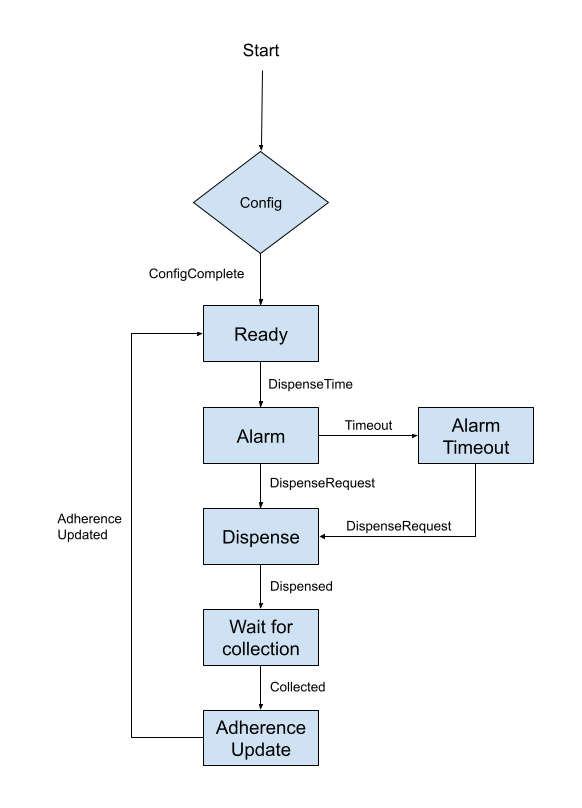
\includegraphics[width=.45\textwidth,height=.45\textheight,keepaspectratio]{project_requirements/FSM.png}
    \caption{Finite State Machine}
    \label{fig:my_label}
\end{figure}

\begin{table}[H] \begin{center} \begin{adjustbox}{max width=\textwidth} \small
\begin{tabular}{|p{0.52\textwidth}|p{0.52\textwidth}|}
 \hline
 \textbf{State} & \textbf{Description}\\
 \hline 
 Config & The device will configure and test all peripherals to ensure they are in working condition and the device can operate successfully. \\
 
 \hline
 Ready & This is a holding period. The device is waiting for the next scheduled dispense time. In this state, the user can change device settings, view current parameters and see the current RTC time. \\
 
 \hline
 Alarm & The device will emit visible and audible alarms to alert the user that their medication is ready to be dispensed. \\
 \hline
  Alarm Timeout & The alarm has either been acknowledged. \\
 \hline
   Dispense & The device will initiate its internal mechanism to perform its dispensing action. \\
 \hline
   Wait For Collection & This is a holding period. A sensor will polled to determine if/when the pouch is collected  \\
 \hline
    Adherence Update & Timestamp the pouch collection/non-collection and store it internally for user reference \\
 \hline
 
 
\end{tabular}\end{adjustbox} \end{center}
\caption{Controlled variables}
\end{table}


% On the fence about including an updated version of this table... maybe if we have the time.
%\subsection{Behaviour Overview}  
%\vspace{-.5cm}
%\begin{align*}
%    PillDispenser &= f(Date/Time, %DispensingSchedule, ManualDispenseRequests, \\ & % PillCollected, PillDispensed, UserInputs, %SachetRollSeated)
%\end{align*}
%
%\begin{table}[ht!]
%\begin{center}
%\begin{adjustbox}{max width=\textwidth}
%\small
%\begin{tabular}{| c | c | c | c |}
%\hline
%  & \multicolumn{3}{c|}{\textit{Results}}\\
% \hline 
 % & \textbf{Dispense} & \textbf{} & %\textbf{Notify}\\
 %\textit{Conditions} & \textbf{Medication} & %textbf{Record data} & \textbf{User}\\
 %\hline 
 %Date/Time = DispensingSchedule & TRUE & TRUE & %TRUE\\
 %\hline
  %Date/Time != DispensingSchedule & FALSE & FALSE & FALSE\\
 %\hline
 % ManualRequest & TRUE & TRUE & FALSE\\
 %\hline
 % !ManualRequest & FALSE & FALSE & FALSE\\
 % \hline
 %  PillCollected & FALSE & TRUE & FALSE\\
 %\hline
 % !PillCollected & FALSE & TRUE & TRUE\\
 %\hline
 %PillDispensed & FALSE & TRUE & FALSE\\
 %\hline
 %!PillDispensed & FALSE & TRUE & TRUE\\
 %\hline
 % UserInputs & X & X & X\\
 %\hline
%\end{tabular}
%\end{adjustbox}
%\end{center}
%\caption{Pill Dispenser Behaviour Table}
%\end{table}


\section{System Requirements}

\subsection{Functional Requirements}
\begin{enumerate}
    \item The dispenser will dispense pouches with 99.9\% effectiveness.
    \item The dispenser must dispense the correct pouch/pouches at the correct time in accordance with a set schedule.
    \item The dispenser will keep track of how many pouches are yet to be dispensed and will tell the user when it is nearly or entirely empty.
    \item The dispenser must verify that the medication was successfully dispensed.
    \item The dispenser must know if and when a dispensed pouch is collected/retrieved by the user and records the event.
    \item The dispenser must keep an accurate real-time clock and must be configurable to the user.
    \item The dispenser must be able to hold and dispense McKesson PACMED strip packages.
    \item The dispenser must notify the user when it is time to take a scheduled medication.
    \item The dispenser must allow the user to manually dispense pouches as necessary. 
    \item The dispenser must allow the user to update the current dispensing schedule as necessary.
    \item The dispenser must store adherence data on local non-volatile memory.
    \item The user must be able to see adherence data via the user interface or through a direct connection to the device (ex. USB).
    \item The dispenser must not damage any pills during the dispensing process.
    \item All moving parts/hazards within the device must be safely concealed to prevent user injury.
    \item The system must be able to identify when a jam occurs and provide instruction to the user.
\end{enumerate}

\subsection{Non-Functional Requirements}
\begin{enumerate}
    \item The dispenser shall dispense a pouch within a reasonable time period ($<$ 15s).
    \item The dispenser shall be easy to set-up with intuitive instructions.
    \item The dispenser shall appear aesthetically pleasing.
    \item The dispenser shall consume minimal power.
    \item The dispenser be small enough to fit on a counter-top.
     \item The dispenser must enter a sleep state if it has had no user interaction for longer than 2 minutes.
\end{enumerate}

\subsection{Requirement Descriptions}
\setlength{\parindent}{0pt} %Automatic indenting turned off past this point.

%-----------------------
\subsubsection*{FR1: The dispenser will dispense pouches with 99.9\% effectiveness.} 
Rationale: Dispensing an improper pouch or damaging the pills inside the pouch can cause serious harm to the user.  
\\\\
Variables of interest:
\begin{itemize}[noitemsep,topsep=0pt]
    \item m\_PillCollected
    \item m\_PillDispensed
    \item m\_DispensingSchedule
    \item c\_AdherenceStatistics
\end{itemize} 
\bigskip
Performance Requirements:
\begin{itemize}[noitemsep,topsep=0pt]
    \item The system must perform all dispensing actions with 99.9\% effectiveness.
\end{itemize}
\bigskip
Normal Operation:
\begin{itemize}[noitemsep,topsep=0pt]
    \item The required pouch is cut open and dispensed at the required time.
\end{itemize}
\bigskip
Undesired Event Handling:
\begin{itemize}[noitemsep,topsep=0pt]
    \item The system has jammed
    \begin{itemize}
        \item The system will stop all current operations and notify the user. The jam must be corrected to continue operation.
    \end{itemize}
    \item Adherence save/load data corrupted.
    \begin{itemize}
        \item The system will notify the user and disable further read/writes.
    \end{itemize}
\end{itemize}
\bigskip

%-----------------------
\subsubsection*{FR2: The dispenser must dispense the correct pouch/pouches at the correct time in accordance with a set schedule.}
Rationale: Dispensing an improper pouch  can cause serious harm to the user.  
\\\\
Variables of interest:
\begin{itemize}[noitemsep,topsep=0pt]
    \item m\_PillDispensed
    \item m\_DispensingSchedule
\end{itemize} 
\bigskip
Performance Requirements:
\begin{itemize}[noitemsep,topsep=0pt]
    \item  The device shall dispense according to the m\_DispensingSchedule variable and detect success/error through the m\_PillDispensed variable.
\end{itemize}
\bigskip
Normal Operation:
\begin{itemize}[noitemsep,topsep=0pt]
     \item The required pouch is cut open and dispensed at the required time.
\end{itemize}
\bigskip
Undesired Event Handling:
\begin{itemize}[noitemsep,topsep=0pt]
    \item The saved schedule data has corrupted
    \begin{itemize}
        \item The system will stop all current operations and notify the user. The user must re-input all dispense times
    \end{itemize}
    \item The system has jammed
    \begin{itemize}
        \item The system will stop all current operations and notify the user. The jam must be corrected to continue operation.
    \end{itemize}
        \item The next pouch in queue is the incorrect pouch for the current dispensing period.
    \begin{itemize}
        \item The system will stop all current operations and notify the user. The pouch will be discarded into a bin internally.
        \item This scenario will become prevalent if a missed dose is encountered.
    \end{itemize}
\end{itemize}
\bigskip

%-----------------------
\subsubsection*{FR3: The dispenser will keep track of how many pouches are yet to be dispensed and will tell the user when it is nearly or entirely empty.}
Rationale: This information will allow the user to plan their next prescription renewal.
\\\\
Variables of interest:
\begin{itemize}[noitemsep,topsep=0pt]
    \item m\_DispensingSchedule
\end{itemize} 
\bigskip
Performance Requirements: 
\begin{itemize}[noitemsep,topsep=0pt]
    \item With the assumed knowledge of the m\_DispensingSchedule, the remaining pouches left will be calculated as dispensing occurs.
\end{itemize}
\bigskip
Normal Operation:
\begin{itemize}[noitemsep,topsep=0pt]
    \item The device will display an audible/visible alarm notifying the user on their low inventory.
\end{itemize}
\bigskip
Undesired Event Handling:
\begin{itemize}[noitemsep,topsep=0pt]
    \item A miscalculation occurs causing an attempted dispense when there is no inventory or the next pouch in queue is not correct.
    \begin{itemize}
        \item The system will check if there is a pouch to dispense and if so, it is the correct pouch. If not, the same event handling will be followed from FR2. 
    \end{itemize}
\end{itemize}
\bigskip

%-----------------------
\subsubsection*{FR4: The dispenser must verify that the medication was successfully dispensed.}
Rationale: Retrieving medication when not desired can cause harm to the user or damage to the device or the strip pack.
\\\\
Variables of interest: 
\begin{itemize}[noitemsep,topsep=0pt]
    \item m\_PillDispensed
    \item c\_AudioVisualAlarm
\end{itemize} 
\bigskip
Performance Requirements:
\begin{itemize}[noitemsep,topsep=0pt]
    \item The system shall monitor the system state through the monitored variables and notify the user when the medication is safe to collect.
\end{itemize}
\bigskip
Normal Operation:
\begin{itemize}[noitemsep,topsep=0pt]
    \item A reflective sensor in the collection area will be polled to detect when a pouch has been dispensed. Once this sensor is triggered, the medication is safe to collect and the user will be notified.
\end{itemize}
\bigskip
Undesired Event Handling:
\begin{itemize}[noitemsep,topsep=0pt]
    \item The system has jammed
    \begin{itemize}
        \item The system will stop all current operations and notify the user. The jam must be corrected to continue operation.
    \end{itemize}
\end{itemize}
\bigskip

%-----------------------
\subsubsection*{FR5: The dispenser must know if and when a dispensed pouch is collected/retrieved by the user and records the event.}
Rationale: Collecting this data will allow the device to store adherence statistics for review by the user.
\\\\
Variables of interest:
\begin{itemize}[noitemsep,topsep=0pt]
    \item c\_AdherenceStatistics
    \item m\_PillDispensed
    \item m\_DateTime
    \item m\_PillCollected
\end{itemize} 
\bigskip
Performance Requirements:
\begin{itemize}[noitemsep,topsep=0pt]
    \item Using the monitored variables, the system shall write to memory the date and time of the collection in a CSV format.
\end{itemize}
\bigskip
Normal Operation:
\begin{itemize}[noitemsep,topsep=0pt]
    \item The device will monitor the collection sensor. If collection is detected, a timestamp in the proper format will be created and written to memory with a dispensed tag. If not collection occurs after a specified timeout a missed dose tag will be attached to the written timestamp.
\end{itemize}
\bigskip
Undesired Event Handling:
\begin{itemize}[noitemsep,topsep=0pt]
    \item A non-dispensing event triggers the collection sensor
    \begin{itemize}
        \item The system will check if a dispensing state had just completed successfully. If not, the trigger would be ignored.
    \end{itemize}
\end{itemize}
\bigskip

%-----------------------
\subsubsection*{FR6: The dispenser must keep an accurate real-time clock.}
Rationale: A non-accurate RTC can cause undesired dispense actions to occur. A configurable RTC will allow the user to set the device time to their local time.
\\\\
Variables of interest:
\begin{itemize}[noitemsep,topsep=0pt]
    \item m\_DateTime
\end{itemize} 
\bigskip
Performance Requirements:
\begin{itemize}[noitemsep,topsep=0pt]
    \item The onboard RTC should tick in reference to the date and time specified by the user.
\end{itemize}
\bigskip
Normal Operation:
\begin{itemize}[noitemsep,topsep=0pt]
    \item On first startup, the device would allow the user to set the current device time to their local time. The RTC time will then be displayed on the UI and tick accordingly.
\end{itemize}
\bigskip
Undesired Event Handling:
\begin{itemize}[noitemsep,topsep=0pt]
    \item RTC clock becomes out-of-sync (e.g. unexpected device shutdown).
    \begin{itemize}
        \item The user will be forced to update the onboard RTC. The device will then ensure the next pouch to dispense is correct and notify accordingly.
    \end{itemize}
\end{itemize}
\bigskip

%-----------------------
\subsubsection*{FR7: The dispenser must be able to hold and dispense McKesson PACMED strip packages.}
Rationale: Ensuring the device is designed to hold the strip packages securely will ensure the package into a undesirable position.
\\\\
Variables of interest:
\begin{itemize}[noitemsep,topsep=0pt]
    \item k\_StripPackageLength
    \item k\_StripPackageWidth
    \item k\_StripPackageHeight
\end{itemize} 
\bigskip
Performance Requirements:
\begin{itemize}[noitemsep,topsep=0pt]
    \item The package should not be put into a undesirable position causing operational errors due to circumstances cause by the enviroment the device is in.
\end{itemize}
\bigskip
Normal Operation:
\begin{itemize}[noitemsep,topsep=0pt]
    \item The device is opened and the user places the package into the device. Closing the device ensures the strip package will remain in place.
\end{itemize}
\bigskip
Undesired Event Handling: N/A
\\\\

%-----------------------
\subsubsection*{FR8: The dispenser must notify the user when it is time to take a scheduled medication.}
Rationale: Without a notification, the user may forget or disregard their medication obligation.
\\\\
Variables of interest:
\begin{itemize}[noitemsep,topsep=0pt]
    \item m\_PillDispensed
    \item c\_AudioVisualAlarm
\end{itemize} 
\bigskip
Performance Requirements:
\begin{itemize}[noitemsep,topsep=0pt]
    \item The system must provide audible/visual alarms to user when desired.
\end{itemize}
\bigskip
Normal Operation:
\begin{itemize}[noitemsep,topsep=0pt]
    \item After a successful dispense occurs, a visible notification will be displayed on the device and an audible tone will be emitted.
\end{itemize}
\bigskip
Undesired Event Handling:
\begin{itemize}[noitemsep,topsep=0pt]
    \item Alarm fails to fire or dismiss.
    \begin{itemize}
        \item The device will perform a soft reset.
    \end{itemize}
\end{itemize}
\bigskip

%-----------------------
\subsubsection*{FR9: The dispenser must allow the user to manually dispense pouches as necessary.}
Rationale: If the user is going to be away from the machine during their dispensing periods, they are still required to take their medication.
\\\\
Variables of interest:
\begin{itemize}[noitemsep,topsep=0pt]
    \item m\_UserInputs
\end{itemize} 
\bigskip
Performance Requirements:
\begin{itemize}[noitemsep,topsep=0pt]
    \item An interaction on the user interface must trigger a dispensing action.
\end{itemize}
\bigskip
Normal Operation:
\begin{itemize}[noitemsep,topsep=0pt]
    \item A press of the manual dispense button on the user interface will force a dispensing action to occur.
\end{itemize}
\bigskip
Undesired Event Handling:
\begin{itemize}[noitemsep,topsep=0pt]
    \item The requested dispense is not performed.
    \begin{itemize}
        \item The undesired event handling from FR4 should be followed.
    \end{itemize}
\end{itemize}
\bigskip


%-----------------------
\subsubsection*{FR10: The dispenser must allow the user to update the current dispensing schedule as necessary.}
Rationale: Dispensing times should be at the convince of the user, not the device.
\\\\
Variables of interest:
\begin{itemize}[noitemsep,topsep=0pt]
    \item m\_DispensingSchedule
\end{itemize} 
\bigskip
Performance Requirements:
\begin{itemize}[noitemsep,topsep=0pt]
    \item The user should be able to retrieve the current state of the monitored variable and configure the values to their needs. The device should store this variable locally.
\end{itemize}
\bigskip
Normal Operation:
\begin{itemize}[noitemsep,topsep=0pt]
    \item The user will trigger the edit dispense times page through a button press. This page will display the current dispense times  along with an edit button for each time. A button press on the edit button will display the increment/decrement time buttons to make the necessary changes.
\end{itemize}
\bigskip
Undesired Event Handling:
\begin{itemize}[noitemsep,topsep=0pt]
    \item Save/load data is corrupted.
    \begin{itemize}
        \item The user will be notified that the data was corrupted and force the user to set new values.
    \end{itemize}
\end{itemize}
\bigskip

%-----------------------
\subsubsection*{FR11:  The dispenser must store adherence data on local non-volatile memory.}
Rationale: Storing the data locally and in non-volatile memory ensures data will be available regardless of unexpected device events. 
\\\\
Variables of interest:
\begin{itemize}[noitemsep,topsep=0pt]
    \item c\_AdherenceStatistics
\end{itemize} 
\bigskip
Performance Requirements:
\begin{itemize}[noitemsep,topsep=0pt]
    \item On change of the monitored variable, the device must store the new data in its local non-volatile memory.
\end{itemize}
\bigskip
Normal Operation:
\begin{itemize}[noitemsep,topsep=0pt]
    \item When a new adherence statistic is available, it will be stored on-board the device.
\end{itemize}
\bigskip
Undesired Event Handling:
\begin{itemize}[noitemsep,topsep=0pt]
    \item Save/load data is corrupted.
    \begin{itemize}
        \item The user will be notified that the data was corrupted. The sector of memory will be cleared.
    \end{itemize}
\end{itemize}
\bigskip

%-----------------------
\subsubsection*{FR12:  The user must be able to see adherence data via the user interface or through a direct connection to the device (ex.  USB).}
Rationale: Once collected the user and/or their caregiver must be able see/extract adherence data so they can gain insight into the user's habits.
\\\\
Variables of interest:
\begin{itemize}[noitemsep,topsep=0pt]
    \item c\_AdherenceStatistics
    \item m\_UserInputs
\end{itemize} 
\bigskip
Performance Requirements:
\begin{itemize}[noitemsep,topsep=0pt]
    \item Data must be displayed on the user interface in a timely manner.
    \item Data must downloaded from the device in a timely manner. 
\end{itemize}
\bigskip
Normal Operation:
\begin{itemize}[noitemsep,topsep=0pt]
    \item While in the ready state the user can access their adherence data by sending a command through the user interface. Likewise, they may initiate a download request from the UI to an external device.
\end{itemize}
\bigskip
Undesired Event Handling:
\begin{itemize}[noitemsep,topsep=0pt]
    \item Adherence data is corrupted
\begin{itemize}
    \item User will be notified that the data is corrupted.
\end{itemize}
\end{itemize}
\bigskip

%-----------------------
\subsubsection*{FR13:  The dispenser must not damage any pills during the dispensing process.}
Rationale: The end user must receive their medication from the system in the same manor in which they would if they have done it themselves.
\\\\
Variables of interest:
\begin{itemize}[noitemsep,topsep=0pt]
    \item c\_DispensingMechanism
\end{itemize} 
\bigskip
Performance Requirements:
\begin{itemize}[noitemsep,topsep=0pt]
    \item The system must accurately cut each pouch along the edge as to reduce chance of blade-pill interaction.
\end{itemize}
\bigskip
Normal Operation:
\begin{itemize}[noitemsep,topsep=0pt]
    \item The pouch is cut and dispensed in such a manor that no pills are damaged.
\end{itemize}
\bigskip
Undesired Event Handling:
\begin{itemize}[noitemsep,topsep=0pt]
    \item Pill is damaged while the pouch is being cut and dispensed.
    \begin{itemize}
        \item The user must be able to retrieve any remaining fragment of the damaged pill from the collection area.
        \item The user must be able to remove the strip package and attempt to re-calibrate.
    \end{itemize}
\end{itemize}
\bigskip

%-----------------------
\subsubsection*{FR14:  All moving parts/hazards within the device must be safely concealed to prevent user injury.}
Rationale: User interacting with the device in a normal manor should not bear a risk of injury.
\\\\
Variables of interest: N/A
\\ \\
Performance Requirements: N/A
\\ \\
Normal Operation:
\begin{itemize}[noitemsep,topsep=0pt]
    \item The device cuts and dispenses pouches internally and does not allow the user to retrieve the pouch until it it safe to do so.
\end{itemize}
\bigskip
Undesired Event Handling: N/A
\\ \\

%-----------------------
\subsubsection*{FR15: The system must be able to identify when a jam occurs and provide instruction to the user.}
Rationale: Knowing when the system has a jam is critical in mitigating potential damage pills and the critical components of the dispensing mechanism.
\\\\
Variables of interest:
\begin{itemize}[noitemsep,topsep=0pt]
    \item m\_PillDispensed
    \item c\_DispensingMechanism
\end{itemize} 
\bigskip
Performance Requirements:
\begin{itemize}[noitemsep,topsep=0pt]
    \item Utilizing the variables of interest the device will identify a jam in a timely manner.
\end{itemize}
\bigskip
Normal Operation:
\begin{itemize}[noitemsep,topsep=0pt]
    \item When a dispensing event is triggered a pill pouch is cut and transported to the collection area.
\end{itemize}
\bigskip
Undesired Event Handling:
\begin{itemize}[noitemsep,topsep=0pt]
    \item Jam is not identified and the device proceeds with the dispensing event.
    \begin{itemize}
        \item An emergency stop option will be available for the user.
    \end{itemize}
\end{itemize}
\bigskip

%-----------------------
\subsubsection*{NFR1: The dispenser shall dispense a pouch within a reasonable time period ($\leq$15s).}
Rationale: Once the user acknowledges the alarm they should not have to wait long for the pouch to be dispensed. Improves user experience.
\\\\
Variables of interest:
\begin{itemize}[noitemsep,topsep=0pt]
    \item m\_PillDispensed
    \item c\_DispensingMechanism
\end{itemize} 
\bigskip
Performance Requirements:
\begin{itemize}[noitemsep,topsep=0pt]
    \item After alarm acknowledgement the pouch must be dispensed within 15 seconds.
\end{itemize}
\bigskip
Normal Operation:
\begin{itemize}[noitemsep,topsep=0pt]
    \item When a scheduled dispense time is reached the system begins to alarm. The user acknowledges the alarm and a pouch is cut and dispensed into the collection area.
\end{itemize}
\bigskip
Undesired Event Handling:
\begin{itemize}[noitemsep,topsep=0pt]
    \item The pouch takes over 15 seconds to dispense.
    \begin{itemize}
        \item The event will be recorded in the system log.
    \end{itemize}
\end{itemize}
\bigskip

%-----------------------
\subsubsection*{NFR2: The dispenser shall be easy to set-up with intuitive instructions.}
Rationale: Users of the product should be given adequate instruction on how to set up the device. Intuitive, easy to understand instructions/set-up processes leave a great first impression of the device on the user.
\\\\
Variables of interest:
\begin{itemize}[noitemsep,topsep=0pt]
    \item m\_UserInputs
    \item m\_StripPackageSeated
    \item c\_SeatedErrorNotifier
\end{itemize} 
\bigskip
Performance Requirements:
\begin{itemize}[noitemsep,topsep=0pt]
    \item Average users will be able to unbox and set-up the device in under 10 minutes.
\end{itemize}
\bigskip
Normal Operation:
\begin{itemize}[noitemsep,topsep=0pt]
    \item Once powered on, the user interface of the device will walk the user step-by-step through set-up, providing feedback throughout the process.
\end{itemize}
\bigskip
Undesired Event Handling:
\begin{itemize}[noitemsep,topsep=0pt]
    \item The system skips the set-up sequence and enters the ready-state.
    \begin{itemize}
        \item The device must have reset functionality that returns it to the set-up state.
    \end{itemize}
\end{itemize}
\bigskip

%-----------------------
\subsubsection*{NFR3: The dispenser shall appear aesthetically pleasing.}
Rationale: Creating a device that users do not find aesthetically pleasing is likely to inhibit user adoption and may encourage them to place the device in low vacancy areas within the home.
\\\\
Variables of interest:
\begin{itemize}[noitemsep,topsep=0pt]
    \item k\_DispenserLength
    \item k\_DispenserWidth
    \item k\_DispenserHeight
\end{itemize} 
\bigskip
Performance Requirements: N/A
\\ \\
Normal Operation: N/A
\\ \\
Undesired Event Handling: N/A
\\
%-----------------------
\subsubsection*{NFR4: The dispenser shall consume minimal power.}
Rationale: The device should not consume more power than necessary preventing unnecessary utility bill increases.
\\\\
Variables of interest: N/A
\bigskip
Performance Requirements:
\begin{itemize}[noitemsep,topsep=0pt]
    \item Peak power consumption of the device will be below 15W.
\end{itemize}
\bigskip
Normal Operation:
\begin{itemize}[noitemsep,topsep=0pt]
    \item Maximum power draw will come from the device while it is alarming, cutting, and dispensing a pouch. When in the ready state for longer than 2 minutes the device will enter a sleep mode to reduce power consumption.
\end{itemize}
\bigskip
Undesired Event Handling:
\begin{itemize}[noitemsep,topsep=0pt]
    \item The system draws a larger than normal current from the power supply.
    \begin{itemize}
    \item The device will monitor power consumption and will enter a safe state when an unexpected power draw event occurs.
    \end{itemize}
\end{itemize}
\bigskip
%-----------------------
\subsubsection*{NFR5: The dispenser be small enough to fit on a counter-top.}
Rationale: Having the device be the same size as a small kitchen appliance improves convenience, and allows for a flexible array of set-up locations.
\\\\
Variables of interest:
\begin{itemize}[noitemsep,topsep=0pt]
    \item k\_DispenserLength
    \item k\_DispenserWidth
    \item k\_DispenserHeight
\end{itemize} 
\bigskip
Performance Requirements:
\begin{itemize}[noitemsep,topsep=0pt]
    \item Footprint of the device should be no larger than the average size toaster (20cm x 30cm approx.)
\end{itemize}
\bigskip
Normal Operation: 
\begin{itemize}[noitemsep,topsep=0pt]
    \item Once set-up the device lives on the kitchen counter, end-table, dresser, etc.
\end{itemize}
\bigskip
Undesired Event Handling: N/A
\\ \\

%-----------------------
\subsubsection*{NFR6: The dispenser must enter a sleep mode if it has had no user interaction for longer than 2 minutes.} 
Rationale: Save energy and preserve the lifespan of user interface components.
\\\\
Variables of interest:
\begin{itemize}[noitemsep,topsep=0pt]
    \item m\_UserInputs
    \item m\_DateTime
\end{itemize} 
\bigskip
Performance Requirements:
\begin{itemize}[noitemsep,topsep=0pt]
    \item Overall power consumption of the device should decrease to the minimum achievable level for basic functionality.
\end{itemize}
\bigskip
Normal Operation:
\begin{itemize}[noitemsep,topsep=0pt]
    \item If the dispenser has been in the ready state for more than 2 minutes without user interaction the device will turn off the user interface while it continues to monitor the time.
\end{itemize}
\bigskip
Undesired Event Handling:
\begin{itemize}[noitemsep,topsep=0pt]
    \item The system does not enter a sleep state.
    \begin{itemize}
        \item The device will monitor its power consumption and identify that an error has occurred.
    \end{itemize}
\end{itemize}
\bigskip

%%%% NEED TO ADD SECTION ABOUT LIKELIHOOD TO CHANGE AND WHY
\subsection{Requirements Likely to Change}
\noindent All requirements not listed below are unlikely to change.

\begin{itemize}
    \item FR12 - The user must be able to see adherence data via the user interface or through a directconnection to the device (ex.  USB).
    \item FR15 - The system must be able to identify when a jam occurs and provide instruction to the user.
    \item NFR1 - The dispenser shall dispense a pouch within a reasonable time period ($<$ 15s) 
    \item NFR6 - The dispenser must enter a sleep state if it has had no user interaction for longer than 2 minutes.
\end{itemize}

\pagebreak
\section{References}

No reference material was used in the creation of this document.

\end{document}